% !TEX TS-program = pdflatex
% !TEX encoding = UTF-8 Unicode
\documentclass[10pt]{article}

% amsmath package, useful for mathematical formulas
\usepackage{amsmath}
% amssymb package, useful for mathematical symbols
\usepackage{amssymb}
\usepackage[english]{babel}
% graphicx package, useful for including eps and pdf graphics
% include graphics with the command \includegraphics
\usepackage{graphicx}

% cite package, to clean up citations in the main text. Do not remove.
\usepackage{cite}

\usepackage{color} 

% Use doublespacing - comment out for single spacing
%\usepackage{setspace} 
%\doublespacing


% Text layout
\topmargin 0.0cm
\oddsidemargin 0.5cm
\evensidemargin 0.5cm
\textwidth 16cm 
\textheight 21cm

% Bold the 'Figure #' in the caption and separate it with a period
% Captions will be left justified
\usepackage[labelfont=bf,labelsep=period,justification=raggedright]{caption}

% Use the PLoS provided bibtex style
\bibliographystyle{plos2009}

% Remove brackets from numbering in List of References
\makeatletter
\renewcommand{\@biblabel}[1]{\quad#1.}
\makeatother


% Leave date blank
\date{}

\pagestyle{myheadings}
%% ** EDIT HERE **


%% ** EDIT HERE **
%% PLEASE INCLUDE ALL MACROS BELOW

%% END MACROS SECTION

\begin{document}

% Title must be 150 characters or less
\begin{flushleft}
{\Large
\textbf{Illumina Sequencing Artifacts Revealed by Connectivity Analysis of Metagenomic Datasets}
}
% Insert Author names, affiliations and corresponding author email.
\\
Adina Chuang Howe$^{1,2}$, 
Jason Pell$^{1}$,
Rosangela Canino-Koning$^{1}$
Rachel Mackelprang$^{3}$
Susannah Tringe$^{3}$
Janet Jansson$^{3,4}$ 
James M. Tiedje$^{1,2}$
C. Titus Brown$^{1,\ast}$
\\
\bf{1} Microbiology and Molecular Genetics, Michigan State University, East Lansing, MI, USA
\\
\bf{2} Department of Plant, Soil, and Microbial Sciences, Michigan State University, East Lansing, MI, USA
\\
\bf{3} Department of Energy (DOE) Joint Genome Institute, Walnut Creek, CA, USA
\\
\bf{4} Lawrence Berkeley National Laboratory, Genomics Division, Berkeley, CA, USA
\\
$\ast$ E-mail: ctb@msu.edu
\end{flushleft}

% Please keep the abstract between 250 and 300 words
\section*{Abstract}
blah blah blah

\section*{Introduction}
Given the rapid decrease in the costs of sequencing, we can now achieve the sequencing depth necessary to study even the most complex environments \cite{Hess:2011p686,Qin:2010p189}.  High throughput, deep metagenomic sequencing efforts in permafrost soil, human gut, cow rumen, and surface water have provided insights into the genetic and biochemical diversity of environmental microbial populations \cite{Hess:2011p686,Iverson:2012p1281,Qin:2010p189} and the extent to which they are involved in responding to environmental changes \cite{Mackelprang:2011p1087}. These metagenomic studies have all leveraged \emph{de novo} metagenomic assembly of short reads to assign sequences to microbial taxa and function.  \emph{De novo} assembly is an advantageous approach to sequence analysis as it reduces the dataset size by collapsing numerous short reads into fewer contigs and provides longer sequences containing multiple genes and operons \cite{Miller:2010p226,Pop:2009p798} making annotation-based approaches more practical.  Furthermore, it does not rely on the availability of reference genomes to enable identification of novel genetic features and draft genomes \cite{Hess:2011p686,Iverson:2012p1281}.

Although \emph{de novo} metagenomic assembly is a promising approach for deep sequencing of metagenomes, it is complicated by the variable coverage of sequencing reads from mixed populations in the environment and their associated sequencing errors and biases \cite{Mende:2012p1262,Pignatelli:2011p742}. Several metagenomic-specific assemblers have been developed to deal with variable coverage communities, including Meta-IDBA \cite{Peng:2011p898}, MetaVelvet, and SOAPdenovo.  These assemblers rely on local models of sequencing coverage to help build assemblies and thus are sensitive to the effects of sequencing errors and biases on coverage estimations of the underlying dataset. The effects of sequencing errors on \emph{de novo} assembly has been demonstrated in simulated metagenomes \cite{Mavromatis:2006p894,Mende:2012p1262,Pignatelli:2011p742}, but these datasets do not incorporate models that are representative of real metagenomic data.  Specifically, these models exclude the presence of known non-biological sequencing biases \cite{GomezAlvarez:2009p1334,Keegan:2012p1336,Niu:2010p1333} which hinder coverage-based assembly approaches.  

In this study, we examine metagenomic datasets for the presence of these artificial sequencing biases, extending previous work to large and complex datasets produced from the Illumina platform. We characterized sequence connectivity in an assembly graph, identifying potential sequencing biases in regions where numerous reads are connected together.  Within metagenomic datasets, we found that there exist highly connective sequences which originate, at least partially, from sequencing artifacts and that these sequences limit approaches to divide or partition large datasets for further analysis, e.g. {de novo} assembly.  Here, we present approaches to identify and characterize these highly connective sequences and examine the effects of removing these sequences on downstream assemblies.

\section*{Results}

\subsection*{Connectivity analysis of metagenome datasets}

\subsubsection*{Presence of a single, highly-connected lump in all datasets}
We selected datasets from three diverse, medium to high diversity metagenomes from the human gut \cite{Qin:2010p189}, cow rumen \cite{Hess:2011p686}, and agricultural soil, representing metagenomes sequenced to various depths (Table 1).  To evaluate the effects of sequencing coverage, we included lower-coverage subsets of the soil metagenome (520 million reads) containing 50 and 100 million reads.  We also included a previously published error-free simulated, metagenome based on a mixture of 112 reference genomes \cite{Pignatelli:2011p742}.

Initially, we evaluated the amount of connectivity between all sequences in each metagenome using an approach similar to the initial step of short read assemblers to identify overlaps of short sequences of length 'k', or k-mers \cite{Peng:2011p898,Simpson:2009p233,Zerbino:2008p665}.  For complex metagenomes, large amounts of memory are required to store reads and their associated sequencing errors in assembly graphs \cite{Hess:2011p686,Mackelprang:2011p1087,Qin:2010p189}.  To overcome this limitation, we constructed a probabilistic representation of the assembly graph using a bloom filter de Bruijn graph representation within fixed memory as previously described (Pell et al, how to cite this?).  

Using this assembly graph representation, we separated reads contributing to disconnected portions of the metagenome assembly graph (e.g., representatives from separate populations in the source environment).  For each metagenome, regardless of origin, we found a single dominant, highly-connected set of sequencing reads which we henceforth refer to as the  ``lump''  of the dataset (Table 1, column 3).  This lump contained the largest subset of connected sequencing reads and varied in size among the datasets, ranging from 5\% of total reads in the simulated metagenome to 75\% of total reads in the human gut metagenome.  For the soil datasets, as sequencing coverage (e.g., the fraction of reads mapped to an assembly) increased from 1.4 to 4.7 to 5.6\%, the lump size increased more dramatically from 7 to 15 to 35\% of all reads, indicating increasingly larger connectivity between sequences with more sequencing.

\subsubsection*{Characterizing the connectivity in the dominant lump}

Given the large number of reads connected within metagenomic lumps (up to 182 and 262 million reads in the soil and human gut datasets, respectively), we quantified the degree of connectivity of sequences within the lump by estimating the average local graph density from each k-mer (k=32 unless otherwise stated) in the assembly graph (See Methods).  Here, local graph density is a measurement of total connected reads within a radius distance.  We observed that sequences in the identified metagenomic lumps were characterized by very high local graph densities, between 22 to 50\% of the total nodes in metagenomic lump assembly graphs had average graph densities greater than 20 (Table 1).  In comparison, 17\% of the total nodes in the simulated lump had an average local graph density greater than 20, and a mixture of the 112 source genomes for the simulated dataset had fewer than 2\% of its nodes with an average graph density greater than 20.  

We next assessed the extent to which graph density varied by position along the sequencing reads.  The degree of position-specific bias of graph densities was estimated by calculating the average local graph density within ten steps of every k-mer by position in each read.  In all environmental metagenomic reads, we observed biases in graph density at the 3'-end region of reads (Figure 1).  In soil metagenomes, we observed the most dramatic biases with local graph density increasing in sequences located at the 3'-end of the reads.  Notably, this bias was not present in the simulated dataset.  

Next, we performed an exhaustive traversal of the assembly graph and identified the specific sequences within dense regions of the assembly graph which consistently contributed to high connectivity.  We observed that this subset of sequences were also found to exhibit position-specific biases within sequencing reads, with the exception of these sequences in the simulated dataset (Figure 1, solid lines).  Similar to local density trends, position-specific biases of these sequences also varied between metagenomes.  As sequencing coverage increased among metagenomes, the amount of 3'-end bias appeared to decrease (e.g., the soils) or inverse (e.g., rumen and human gut).

\subsection*{Effects of removing highly connective sequences on assembly}

\subsubsection*{Removal of highly connective sequences enables partitioning of metagenome}
Given that highly connective sequences exhibited position-specific biases associated with sequences of non-biological origin, we assessed the effects of their removal from reads in metagenomic lumps.  We found that by removing these k-mers, we could effectively break apart metagenomic lumps, and the resulting largest partition of connected reads in each metagenome was reduced to less than 7\% of the total reads in the lump.  As a consequence of partitioning the metagenomic lump, we were able to greatly reduce assembly requirements.  Compared to unfiltered datasets which required greater than 100 GB and 100 hours in the case of the largest soil metagenome (Table 2), all partitioned datasets could be assembled in less than 2 GB of memory and less than 1 hour using multiple nodes. 

\subsubsection*{Removal of highly connective sequences resulted in minimal losses of reference genes}
To explore the extent to which the identified highly-connective sequences impacted assembly, we first evaluated the effects of the removing these sequences from reads in the simulated lump and its resulting assemblies.  The assembly of the reads in the original, unfiltered simulated lump and that of the reads remaining after removing highly connective sequences (the filtered assembly) were compared for three assemblers:  Velvet, Meta-IDBA, and SOAPdenovo.  Based on the total assembly length of contigs greater than 300 bp, filtered assemblies of the simulated metagenome resulted in a loss of between 4 - 16\% of total assembly length (Table 2).   In general, the filtered assemblies contained fewer total contigs than unfiltered assemblies, and the maximum contig size increased in the Velvet assembly but decreased in the Meta-IDBA and SOAPdenovo assemblies.  Direct comparisons of the unfiltered and filtered assemblies found that the filtered assemblies comprised on average 88\% of the unfiltered assemblies, and the unfiltered assemblies contained nearly all, 96\%, of the filtered assembled sequences.  Despite the removal of over 3\% of the total unique 32-mers in the simulated metagenome, the resulting filtered assemblies resulted in only a loss of 0.1 - 0.6\% of annotated original reference genes (Tables 1 and 2). 

We next evaluated the effects of using similar approaches on metagenomic datasets.  Similar to the simulated assemblies, the removal of highly connective sequences for all metagenomes and assemblers resulted in a loss of total number of contigs and assembly length (Table 2).  In general, filtered assemblies were largely contained within unfiltered assemblies and comprised 51-88\% of unfiltered assembly.   The observed changes in metagenomic assemblies were difficult to evaluate as the source genomes to these datasets are unknown, and a loss in assembly length may actually be beneficial due to the elimination of contigs which incorporated sequencing artifacts.  To aid in this evaluation, we used the previously published set of rumen draft genomes from \emph{de novo} assembly efforts of high abundance sequences in the rumen metagenome \cite{Hess:2011p686}.  Overall, we found that removal of highly connective sequences from the rumen dataset resulted in 1-3\% loss of sequences which matched to draft reference genomes (Table 2).  

\subsubsection*{Unfiltered assemblies contained only a small fraction of highly connective sequences}
To further study the effects of highly connective sequences, we examined their incorporation into unfiltered assemblies.   Overall, less than 1\% of highly connective sequences were incorporated by any assembler, the maximum was 3-4\% in the Velvet and Meta-IDBA assemblies of the human gut dataset (Table 1 and 3).  Each assembled contig was divided into equal length bins (the size of bins was dependent on the total length of the contig) and examined for the presence of the previously identified highly connective sequences.  We found that contigs, especially in assemblies from Velvet and Meta-IDBA, incorporated a larger fraction of these sequences at its ends relative to other binned positions (Figure 3).  The SOAPdenovo assembler incorporated fewer of the highly connective sequences into its assembled contigs; none of these sequences in the simulated dataset were assembled, and only 41 in the small soil dataset.  For the human gut metagenome assemblies, millions of the highly connective sequences were incorporated into assembled contigs, comprising nearly 4\% of all assembled sequences on Velvet contig ends (Figure 4, suggestion to move to supp figures).

\subsubsection*{Identifying origins of highly connective sequences in known reference databases}

For the simulated metagenome, we could identify the source of highly connective k-mers using available reference genomes. Reference genes with multiple perfect alignments to highly connective k-mers present in the dataset a minimum of 50 times were identified (Table 4).  Many of these sequences were from well-conserved housekeeping genes involved in protein synthesis, cell transport, and signaling.  To determine possible biological sources of highly connective sequences within real metagenomes, we compared the sequences shared between the soil, rumen, and human gut metagenomes.  For these 7,586 shared sequences (32-mers), we identified the closest reference protein from the NCBI-nr database requiring complete sequence identity.  Only 1,018 sequences (13\%) matched existing reference proteins, and many of the annotated sequences matched multiple conserved protein sequences from multiple genomes.  The top five proteins conserved in greater than 3 genomes are shown in Table 4, and largely encode for genes involved in protein biosynthesis, DNA metabolism, and biochemical cofactors (Table 5).

A potential cause of artificial high connectivity within metagenomes is the presence of high abundance sequences.  Thus, we identified the subset of highly connective k-mers which were also present with an abundance of greater than 50 within each metagenome and their location in sequencing reads (Figure 2, dotted lines).   These high abundance k-mers comprised a very small proportion of the identified highly connective sequences, less than 1\% in the soils, 1.5\% in the rumen, and 6.4\% in the human gut metagenomes, but the position-specific biases of these sequences were very similar to the biases of the larger set of highly connective k-mers.

To identify consistent patterns within sequences causing position-specific biases, we examined the abundance of distribution 5-mers contained within the high abundance subset of each dataset's highly connective 32-mers.   There were significantly fewer 5-mers in the simulated sequences compared to those in metagenomes: 336 5-mers in the simulated and 425,572 to 221,085,228 in the small soil and human gut datasets, respectively.  We examined the distribution of the abundance of these 5-mers, evaluating any significant presence of specific 5-mers.  In the simulated dataset, the top ten most abundant unique k-mer made up 75\% of the total 5-mers; in contrast, in the metagenomes, the top ten most abundant 5-mers comprised less than 10\% of the total 5-mers.  When the 5-mers in each metagenome dataset were ranked from highest to lowest abundance, all sequences represented an even distribution of total cumulative k-mers, and the opposite trend is observed in the simulated dataset where the majority of 5-mers are among the most abundant.

\section*{Discussion}

\subsection*{Sequencing artifacts are present in highly connected sequences}

Through assessing the connectivity of reads in several metagenomes, we identified a disproportionately large subset of reads which were connected together within an assembly graph, hereafter referred to as the ``lump'' in each metagenome.  The total number of reads in metagenomic lumps (7-75\% of reads) was significantly larger than that of simulated dataset (5\% of reads) (Table 1).  As the simulated dataset contains no errors, its observed connectivity represents conserved sequences within a single genome or between multiple genomes (specific genes identified in Table 4).  The larger size of the highly connective lump within the soil, rumen, and human gut metagenomes suggests that anomalous, non-biological connectivity may be present within these lumps.  Interestingly, in the soil metagenomes, we observed that the amount of connectivity nearly doubled with less than a 5\% increase of sequencing coverage.  When sequencing coverage increased slightly from 4.7 to 5.6\% in the medium and large soil metagenomes, the number of reads connected in the lump grew significantly from 15 million to 182 million.  Given the very high diversity and very low coverage of these soils, the magnitude of the observed increases in connectivity seemed unlikely from biological sources, further supporting the presence of sequencing biases within these datasets.  

If sequencing biases were present within these metagenomes, we would expect to observe that the metagenomic lumps would consist not only of artificial sequences but also sequences from reads which would be ``preferentially attached'' \cite{Barabasi:1999p1083}.  Consider that there is an original set of highly connecting ``X'' sequences in a lump.  These sequences would recruit a number of connective ``Y'' reads into the lump.  These recruited ``Y'' reads would then recruit more ``Z'' reads into the lump which would not necessarily connect to the original "X" reads.  In error-free datasets, we would observe this preferential attachment phenomenon as a linear increase of lump size with increasing sequencing coverage.  In the case of the presence of highly-connective sequencing biases, however, we'd observe that preferential attachment would cause dramatic increases in the number of recruited ``Y'' and ``Z'' reads, as is observed in the soil datasets.   

To more rigorously demonstrate the presence of artifacts within our datasets, we considered that the sequencing of metagenomes is a random process and consequently any position-specific bias within sequencing reads is unexpected and non-biological.   For the metagenomes studied here, we used two approaches to examine characteristics of connectivity correlated to specific positions within sequencing reads.  First, we measured the connectivity of sequences at specific positions within reads by calculating local graph density.  Next, we identified the specific k-mers which were consistently present in highly dense regions of the assembly graph and evaluated their location within sequencing reads.  When these approaches were applied to the simulated dataset, we observed no position-specific trends when assessing either local graph density (Figure 1) or highly connective k-mers (Figure 2, solid lines) as is consistent with the lack of sequencing errors and biases in this dataset.  In all real metagenomes, however, we identified position-specific trends in measurements of both local graph density and the location of highly connective sequences, clearly indicating the presence of artificial sequences.  Although present in all metagenomes, the direction of the bias varied between soil, rumen, and human gut datasets, especially for the position-specific presence of identified highly connective sequences.  It is likely that there is a larger presence of indirectly preferentially attached reads which are connected to high coverage sequences of biological origins in higher coverage datasets, such as the rumen and human gut.  This preferential attachment of such reads would result in increasing the number of total reads and consequently the decrease the total fraction of highly connective k-mers (Figure 2, y-axis).  This trend is observed in the decreasing fractions of highly connective sequences at the 3' end of reads as sequencing coverage increased in the small, medium, to large soil metagenomes and in the soil, rumen, to human gut metagenomes (Figure 2).

\subsection*{Assessing the validity of removing highly connective sequences from metagenomes}
\subsubsection*{Highly connective sequences are difficult to assemble}
As is apparent from conserved biological sources of high connectivity within the simulated metagenome, not all the observed connectivity within real metagenomes is artificial, and our approaches are limited in that they cannot differentiate between sequencing artifacts and sources of real biological connectivity.  Regardless of the origin of highly connective sequences, we suspected that these sequences would challenge assemblers which rely on resolving the complex "lump" in the assembly graph.  Indeed, very few highly connective sequences with abundances greater than 50 were incorporated into any assembly (Table 3) and those which were assembled were often disproportionately placed at the ends of contigs (Figure 3), suggesting that assembly could often not extend beyond these sequences.  Although this trend was observed for all assemblers, it was more prevalent in the Velvet and Meta-IDBA assemblers, highlighting differences in assembler heuristics.  

\subsubsection*{Removing highly connective sequences enabled more efficient assembly of partitioned reads}
Given that these sequences were found to have position-specific biases within reads and challenged multiple assemblers, we assessed the effects of removing them for the assembly of metagenomic lumps.  We found that the removal of these highly connective sequences had two key advantages:  first, it removed artificial sequences which should not be assembled, and second, it resulted in the dissolution of the high connectivity within the metagenomic lump and consequently allowed for the partitioning of all metagenomes.  We compared the combined assembly of the partitioned sets of filtered reads to the original lump dataset with several assemblers.  For the partitioned reads, we were able to assemble subsets of reads in parallel, resulting in significantly reduced time and memory requirements for assembly (Table 2).  In the case of the largest soil metagenome (containing over 500 million reads), we could not complete the Meta-IDBA assembly of the unfiltered reads in less than 100 GB of memory, but after removing highly connective sequences and partitioning, the assembly could be completed in less than 2 GB of memory.  Using partitioned sets of reads for all metagenomes, we were also able to efficiently complete multiple k-mer length assemblies (demonstrated with Velvet) and subsequently merge resulting assembled contigs.  For unfiltered datasets, this was previously either impossible (due to memory requirements) or impractical (due to time).   

We used consistent parameters (i.e. k-length, estimations of coverage, etc.) to compare assemblies, but it is often beneficial to optimize these values to characteristics of the underlying dataset.  Partitioning metagenomic reads based on connectivity effectively divides the cumulative environmental dataset into subsets representing fragments from different genomes.  Thus, partitioning enables optimization for a single population subset (rather than a community metagenome) for assembly and many other analyses (i.e. binning, annotation, SNP identification).  Additionally, because the partitions are manageable in size, it is practical to complete multiple assemblies to evaluate different assemblers and/or assembly parameters.  As metagenome datasets grow increasingly larger, this ability to efficiently analyze datasets and/or evaluate multiple assemblies will be increasingly important.

\subsubsection*{Removal of highly connective sequences prior to assembly did not result in significant loss of reference genes}
The advantages of removing highly connective sequences must be balanced against consequences to resulting assemblies.  We compared several metagenome assemblies before and after the removal of these sequences.   Comparing the simulated dataset's assemblies, the removal of highly connective sequences resulted in very little loss of annotated reference genes (less than 1\%) and a similar assembly compared to the unfiltered data (~85\% similarity), supporting the removal of these highly connective sequences especially for gains in assembly efficiency.  For the rumen metagenome, we performed a partial evaluation of the assemblies using available draft reference genomes.   Similar to the simulated assemblies, we observed only a small loss (less than 3\%) of rumen reference genomes assembled (Table 2).  In general, for all metagenomes, we observed ~25\% loss in assembly after removing highly connective sequences, much more than observed in assemblies of reference genes and genomes in the simulated and rumen datasets.  Some of this loss is likely beneficial, resulting in the removal of sequencing artifacts; it is also possible that our approach removes sequences which can accurately be assembled but cannot be distinguished due to lack of reference genomes.  However, without the removal of these sequences, many of the assemblies of the larger metagenomes would not be practical. 

\subsection*{Highly connective sequences do not match known reference sequences}

We attempted to identify any biological characteristics of highly connective sequences.  Among these sequences in the simulated dataset and those shared by all metagenomes, we identified only a small fraction (13\% in simulated and less than 7\% in metagenomes) which matched reference genes, mostly associated with housekeeping functions (Tables 4 and 5).  This suggests that the remaining sequences are either not present in known reference genes (i.e., conserved non-coding regions) or originate from non-biological sources and supports the removal of these sequences for typical assembly and annotation pipelines, where assembly is often followed by the identification of protein coding regions.

Speculating that many of the highly connective sequences originated from high abundance reads (possibly originating from biological sources of high connectivity or sequencing biases), we identified characteristics of the most abundant subset of sequences.  We found that these sequences (present greater than 50x) displayed similar trends for position-specific biases compared to their respective sets of highly connective sequences (Figure 2), indicating that they are contribute significantly as sequencing biases.  We attempted to identify signatures in the the abundant, highly connective sequences of the simulated and metagenomic datasets.  In the simulated dataset, we found that the total number of unique 5-mers was significantly lower than that in metagenomes and that the most abundant of these 5-mers comprised the large majority of the total.  This result is consistent with the identification of conserved biological motifs in the simulated dataset which would result in a small number of highly abundant sequences.  In contrast, within metagenomic data, we found that these sequences are evenly distributed and random in metagenomes (Figure 5), making them difficult to identify and evaluate.  Currently, we are evaluating a promising approach to improve the identification and removal of probable sequencing artifacts based on targeting high abundance sequencing. 

\section*{Conclusion}

As datasets from NGS technologies continue to increase in size, current analysis approaches are no longer adequate.  In this study, we characterize the connectivity of sequences in several metagenomes to better understand how we can improve approaches towards {de novo} metagenomic assembly.  We demonstrate the existence of extremely highly connective sequences within several metagenomes and show that they are comprised of sequencing artifacts.  These sequences add erroneous diversity and high coverage to datasets and significantly increase memory requirements for assembly.  We show that assemblers are challenged by these sequences and that their removal results in comparable assemblies and enables partitioning of complex metagenome assembly graphs into disconnected subsets, allowing low-memory execution of previously impractical to complete assemblies.  Our analysis provides an understanding of the nature of highly connective sequences in metagenomes and suggests that their removal is an important first step for scalable \emph{de novo} assembly.  This study highlights the importance of re-evaluating the nature of new sequencing data for both accurate and efficient downstream analysis approaches. 

\section*{Methods}

\subsection*{Metagenomic datasets}
All datasets, with the exception of the agricultural soil metagenome, originate from previously published datasets. Rumen-associated sequences (Illumina) were randomly selected from the rumen metagenome available at ftp://ftp.jgi-psf.org/pub/rnd2/Cow\_Rumen \cite{Hess:2011p686}. Human-gut associated sequences (Illumina) of samples MH0001 through MH0010 were obtained from 
ftp://public.genomics.org.cn/BGI/gutmeta/ Raw\_Reads \cite{Qin:2010p189}.  The simulated high complexity, high coverage dataset was previously published \cite{Pignatelli:2011p742}.  All reads used in this study, with the exception of those in simulated metagenome, were quality-trimmed for Illumina's read segment quality control indicator, where a quality score of 2 indicates that all subsequent regions of the sequence should not be used. After quality-trimming, only reads with lengths greater than 30 bp were retained. All quality trimmed datasets, including the previously unpublished agricultural soil metagenome, are available on a public Amazon EC2 snapshot, XXX. (temporarily on scratch hpc:/mnt/scratch/howead/to-transfer-to-amazon/.)  The sequencing coverage of each metagenome was estimated as the fraction of reads which could be aligned to assembled contigs with lengths greater than 500 bp.  For the coverage estimates, an assembly of each metagenome was performed using Velvet (v1.1.05) with the following parameters:  K=33, exp cov=auto, cov cutoff=0, no scaffolding.  Reads were aligned to assembled contigs with Bowtie (v0.12.7), allowing for a maximum of two mismatches.  

\subsection*{Lightweight, compressible de Bruijn graph representation}
We used a lightweight probabilistic de Bruijn graph representation to explore k-mer connectivity of the assembly graph (cite PNAS paper, software available at https://github.com/ctb/khmer). The de Bruijn graph stores k-mer nodes in Bloom filters and keeps edges between nodes implicitly.  For metagenomes in this study, we used 4 x 48e9 bit bloom filters to store connectivity of the assembly graphs.  We partitioned disconnected subsets of the assembly graph, and the set of the largest number of reads which were connected in the assembly graph is referred to above as a single, highly-connected lump.  Data and examples of scripts used for this analysis are available on the Amazon EC2 public snapshot:  data-in-paper/lumps and method-examples/0.partitioning-into-lump.

\subsection*{Local graph density and identifying highly-connected k-mers}
We implemented a systematic traversal algorithm to identify highly connected components of the assembly graph.  Waypoints were labeled to cover the graph such that they are a minimum distance of L apart. Originating from a waypoint, all k-mers (throughout the study k=32 unless otherwise stated) were systematically and exhaustively traversed within a region that is the distance N.  The local graph density was calculated as the number of X k-mers reachable within a distance of N nodes (k-mers) divided by the distance N.  In this study, N was equal to 10 nodes within the assembly graph.  For the largest metagenomes, the human gut and large soil datasets, local graph density was calculated on a representative subset of reads due to computational limitations.  To identify specific highly-connective sequences within the lump assembly graphs, graph traversal to a distance of 40 nodes was attempted from marked waypoints.  If more than 200 k-mers were found within this traversal were identified, all k-mers within this traversal were identified as candidates for highly connective sequences.  If the same k-mers were consistently identified in other graph traversals, up to five times, the k-mer was flagged as a highly connective sequence.  Aligning theses k-mers to original sequencing reads, we identified the position-specific location of these k-mers.  Data and examples of scripts used for this analysis are available on the Amazon EC2 public snapshot: data-in-paper/density-bias, data-in-paper/hc-kmer-bias, method-examples/1.density-analysis, method-examples/2.identifying-hc-kmers, and method-examples/3.hc-kmer-analysis.

To identify the sources of highly connective k-mers identified in the simulated metagenome, these sequences were aligned against the reference genes originating from the 112 source genomes using Bowtie (v0.12.7) requiring exact matches.   Highly connective k-mers shared between all the metagenomes were also aligned against the NCBI non-redundant genome database (ftp://ftp.ncbi.nih.gov/blast/db, March, 1, 2011) using blastn \cite{Altschul:1990p1335} and requiring an exact match over the entire k-mer.  Genes which matched highly connective sequences and were conserved among genome(s) were identified (Tables 4 and 5).

We also identified the subset of highly connective k-mers which were present at greater than 50 times within lumps. Data used for this analysis are available on the Amazon EC2 public snapshot: data-in-paper/lumps/HC-kmers/HA-HC-kmers and method-examples/4.abundant-hc-kmers. These high abundance, highly connective sequences were aligned to sequencing reads to demonstrate position specific biases as described above.   We evaluated the existence of short k-mer (k=5) motifs within high abundance, highly connective k-mers which did not have an exact match to the NCBI non-redundant database.  Each identified 32-mer was broken up into shorter 5-mers, and the frequency of each unique 5-mer was calculated.  Next, each unique 5-mer was ranked based on its abundance, from high to low, and the cumulative percentage of total 5-mers is shown in the resulting rank-abundance plot (Figure 5).
  
\subsection*{\emph{De novo} metagenomic assembly}

The lump within each dataset was assembled and referred to as the ``unfiltered assembly''.  Additionally, highly connective sequences identified as described above were were trimmed from sequencing reads and the remaining reads partitioned and assembled, resulting in the ``filtered assembly''.  \emph{De novo} metagenomic assembly of reads was completed with Velvet (v1.1.02) with the following parameters: velveth -short -shortPaired (if applicable to the dataset) and velvetg -exp\_cov auto -cov\_cutoff 0 -scaffolding no \cite{Zerbino:2008p665}.  For the small and medium soil, rumen, and simulated datasets, Velvet assemblies were performed at K=25-49, resulting contigs were dereplicated to remove contigs with 99\% similarity using CD-HIT (v 4.5.6, \cite{Li:2001p1337}), and final contigs were merged with Minimus (Amos v3.1.0, \cite{Sommer:2007p1253}).  For the largest soil and human gut metagenomes, assemblies were performed at only K=33 due to the size of the datasets and memory limitations.  Additional assemblies were performed with meta-IDBA (v0.18) \cite{Peng:2011p898} : --mink 25 --maxk 50 --minCount 0 and with SOAPdenovo:  -K 31 -p 8  max\_rd\_len=200 asm\_flags=1 reverse\_seq=0.  After removal of highly connective k-mers in metagenomic lumps, each filtered lump was partitioned into separate disconnected subgraphs.  Multiple subgraphs were grouped together such that assembly could be performed in parallel on groups of sequences.  Identical assembly parameters and methods as described above were used for these assemblies.  Unfiltered and filtered assemblies were compared using the total number of contigs, total assembly length, and maximum contig size.  Additional, the coverage of each assembly was calculated through estimating the average base pair coverage of the BLAST alignment of each assembly to one another (E-value greater than 10$^{-5}$) or, in the case of the simulated and rumen assemblies, to reference genomes.  The simulated and rumen reference genomes were previously published in \cite{Hess:2011p686} and \cite{Pignatelli:2011p742}, respectively.  Resulting assemblies are available on the Amazon EC2 public snapshot: /data-in-paper/assembly*.

We examined incorporation and the location of the identified high abundant, highly connecting k-mers within assembled contigs.  Incorporation of these sequences was evaluated by dividing assembled contigs into words of 32 bp length and identifying exact matches between sequences and contig fragments.  The location of these k-mers within assembled unfiltered contigs was examined by dividing each contig into 100 equally-sized regions.  The fraction of highly-connecting k-mers which aligned exactly to each region was calculated for each metagenome. Data and examples of scripts used for this analysis are available on the Amazon EC2 public snapshot: method-examples/5.hc-kmer-contigs/.



\bibliography{artifacts-bib}


\pagebreak

\begin{table}
\center{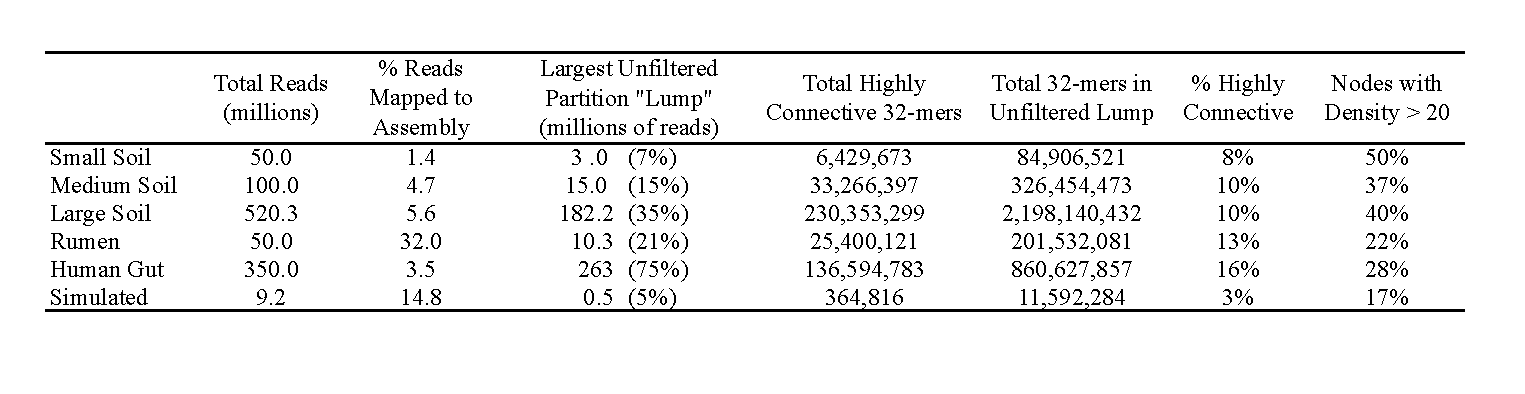
\includegraphics[width=\textwidth,height=\textheight,keepaspectratio]{./Figures/table1.pdf}}
\caption{The original size and proportion of highly connective 32-mers in the largest subset of partitioned reads (``lump'') in several medium to high complexity metagenomes.  Read coverage was estimated with the number of aligned sequencing reads to Velvet-assembled contigs (K=33).  The dominant lump, or largest disconnected component of each metagenome assembly graph, was found to contain highly connecting k-mers responsible for high local graph density.}
\end{table}

\begin{table}
\center{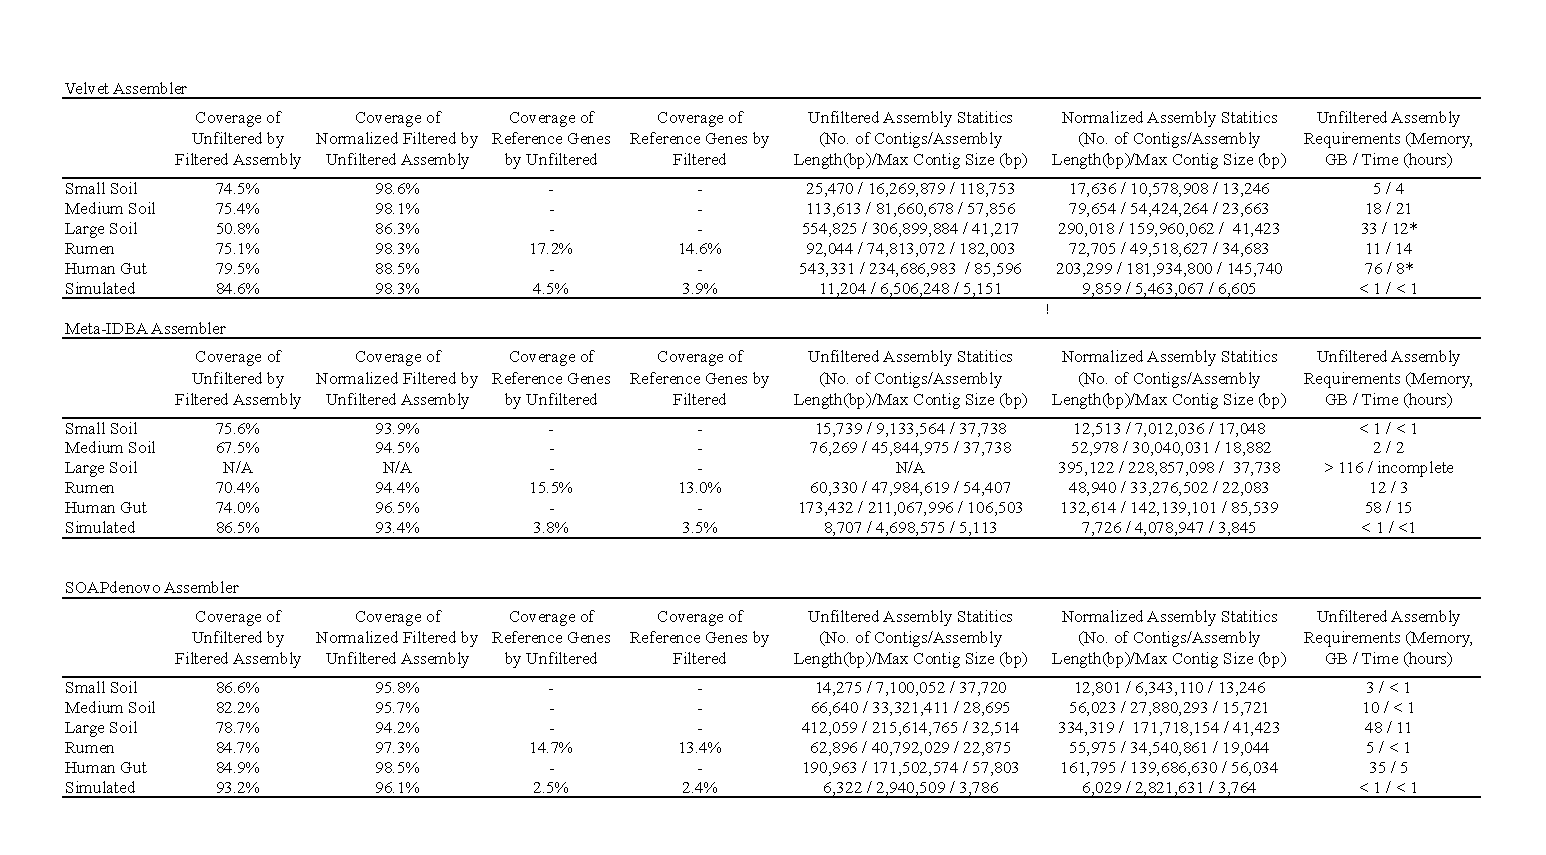
\includegraphics[width=5in]{./Figures/table2-assemblies.pdf}}
\caption{Comparison of unfiltered and filtered assemblies of various metagenome lumps using Velvet, SOAPdenovo, and Meta-IDBA assemblers.  Assemblies were aligned to each other, and coverage was estimated (columns 1-2).  Simulated and rumen assemblies were aligned to available reference genes/genomes (columns 3-4).  Total number of contigs, assembly length, and maximum contig size was estimated for each assembly, as well as memory and time requirements of unfiltered assembly (columns 5-7).  Filtered assemblies required less than 2 GB of memory.  Velvet assemblies of the unfiltered human gut and large soil datasets (marked as *) could only be completed with K=33 due to computational limitations.  The Meta-IDBA assembly of the large soil metagenome could not be completed in less than 100 GB.}
\end{table}

\begin{table}
\center{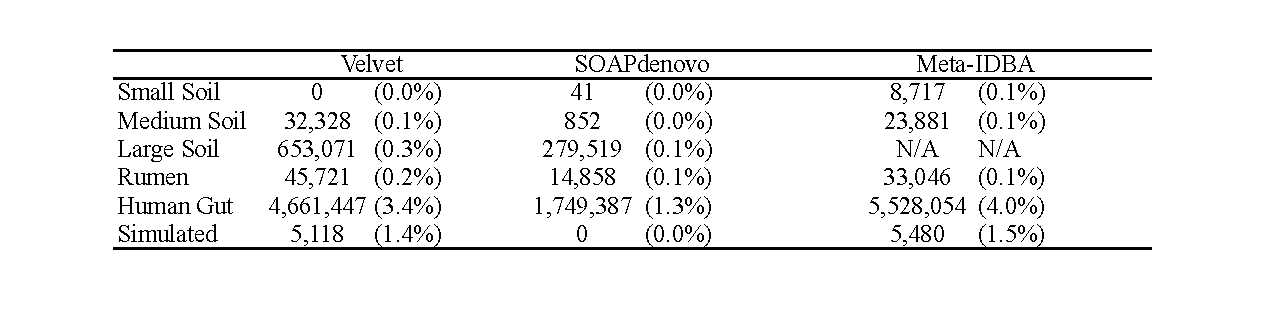
\includegraphics[width=5in]{./Figures/stoptag-table.pdf}}
\caption{Total number of abundant (greater than 50x), highly connective sequences incorporated into unfiltered assemblies (percentage of total highly connective sequences).}
\end{table}

\begin{table}
\center{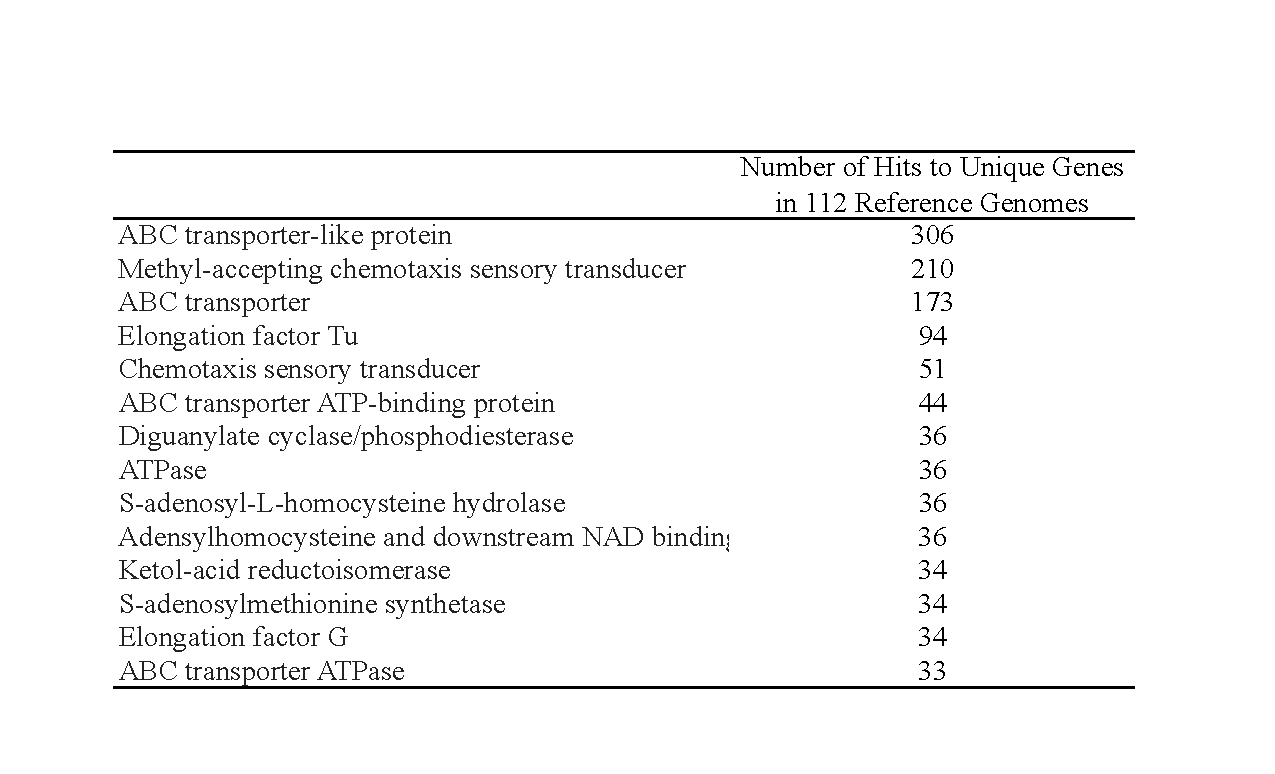
\includegraphics[width=5in]{./Figures/table3-simulated-stoptags.pdf}}
\caption{Annotation of highly-connecting sequences from the simulated metagenome with most hits to conserved genes within the 112 reference genomes \cite{Pignatelli:2011p742}.}
\end{table}

\begin{table}
\center{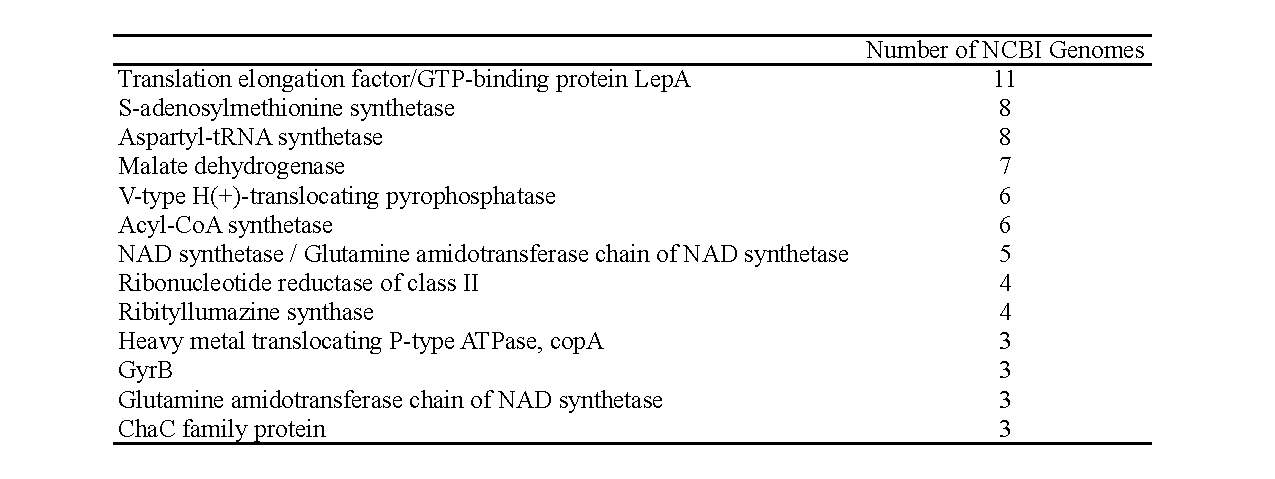
\includegraphics[width=5in]{./Figures/table4-overlap.pdf}}
\caption{Annotation of highly-connecting sequences to conserved nucleotide sequences originating from 3 or more reference genomes.  Shown are protein annotations whose nucleotide sequences matched 3 or more highly-connecting sequences shared in the three soil, rumen, and human gut metagenomes.}
\end{table}

\begin{figure}
\center{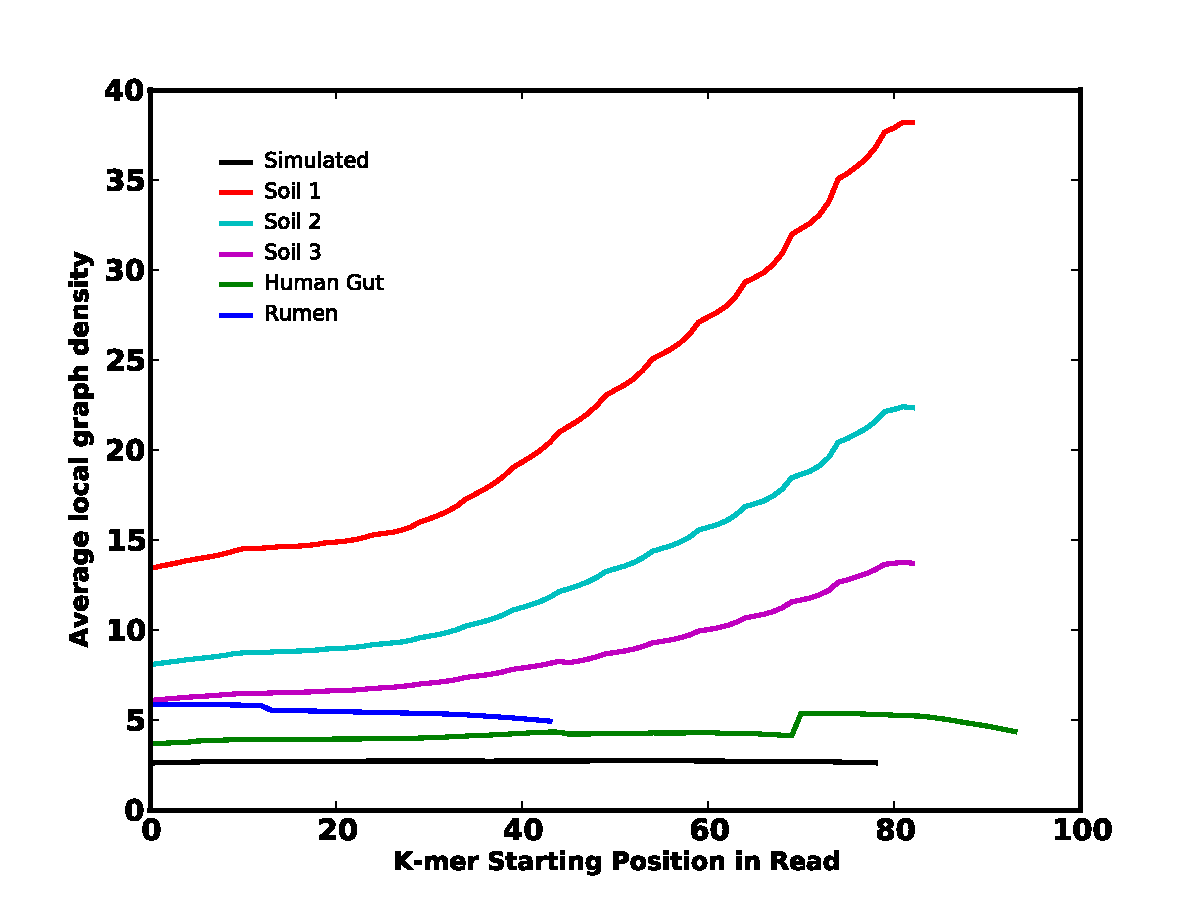
\includegraphics[width=5in]{./Figures/figure1-density.pdf}}
\caption{The extent to which average local graph density varies by read position is shown for the lump of various datasets.}
\end{figure}

\begin{figure}
\center{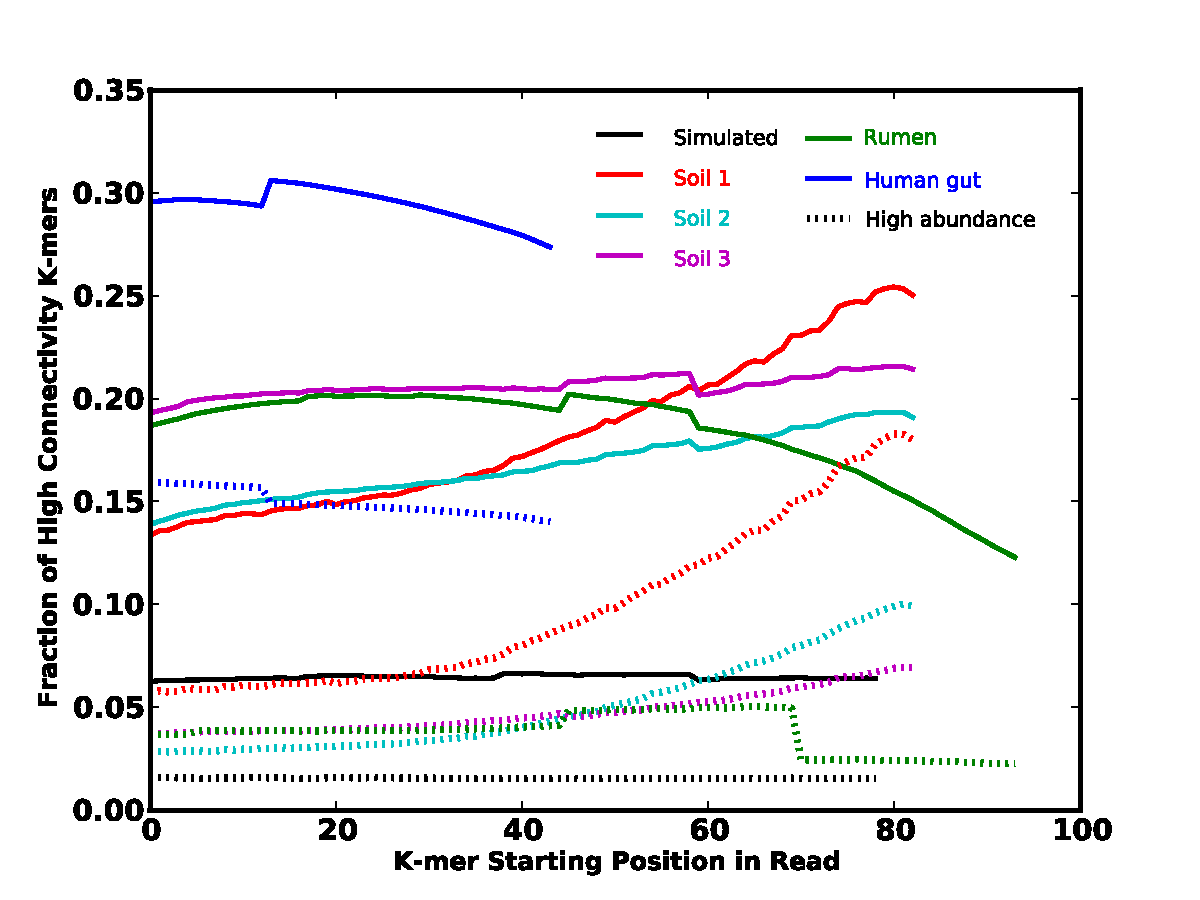
\includegraphics[width=5in]{./Figures/figure2-hckmers.pdf}}
\caption{The extent to which highly-connecting k-mers (solid lines) and the subset of highly abundant (greater than 50) k-mers (dashed lines) are present at specific positions within sequencing reads for various metagenomes.}
\end{figure}

\begin{figure}
\center{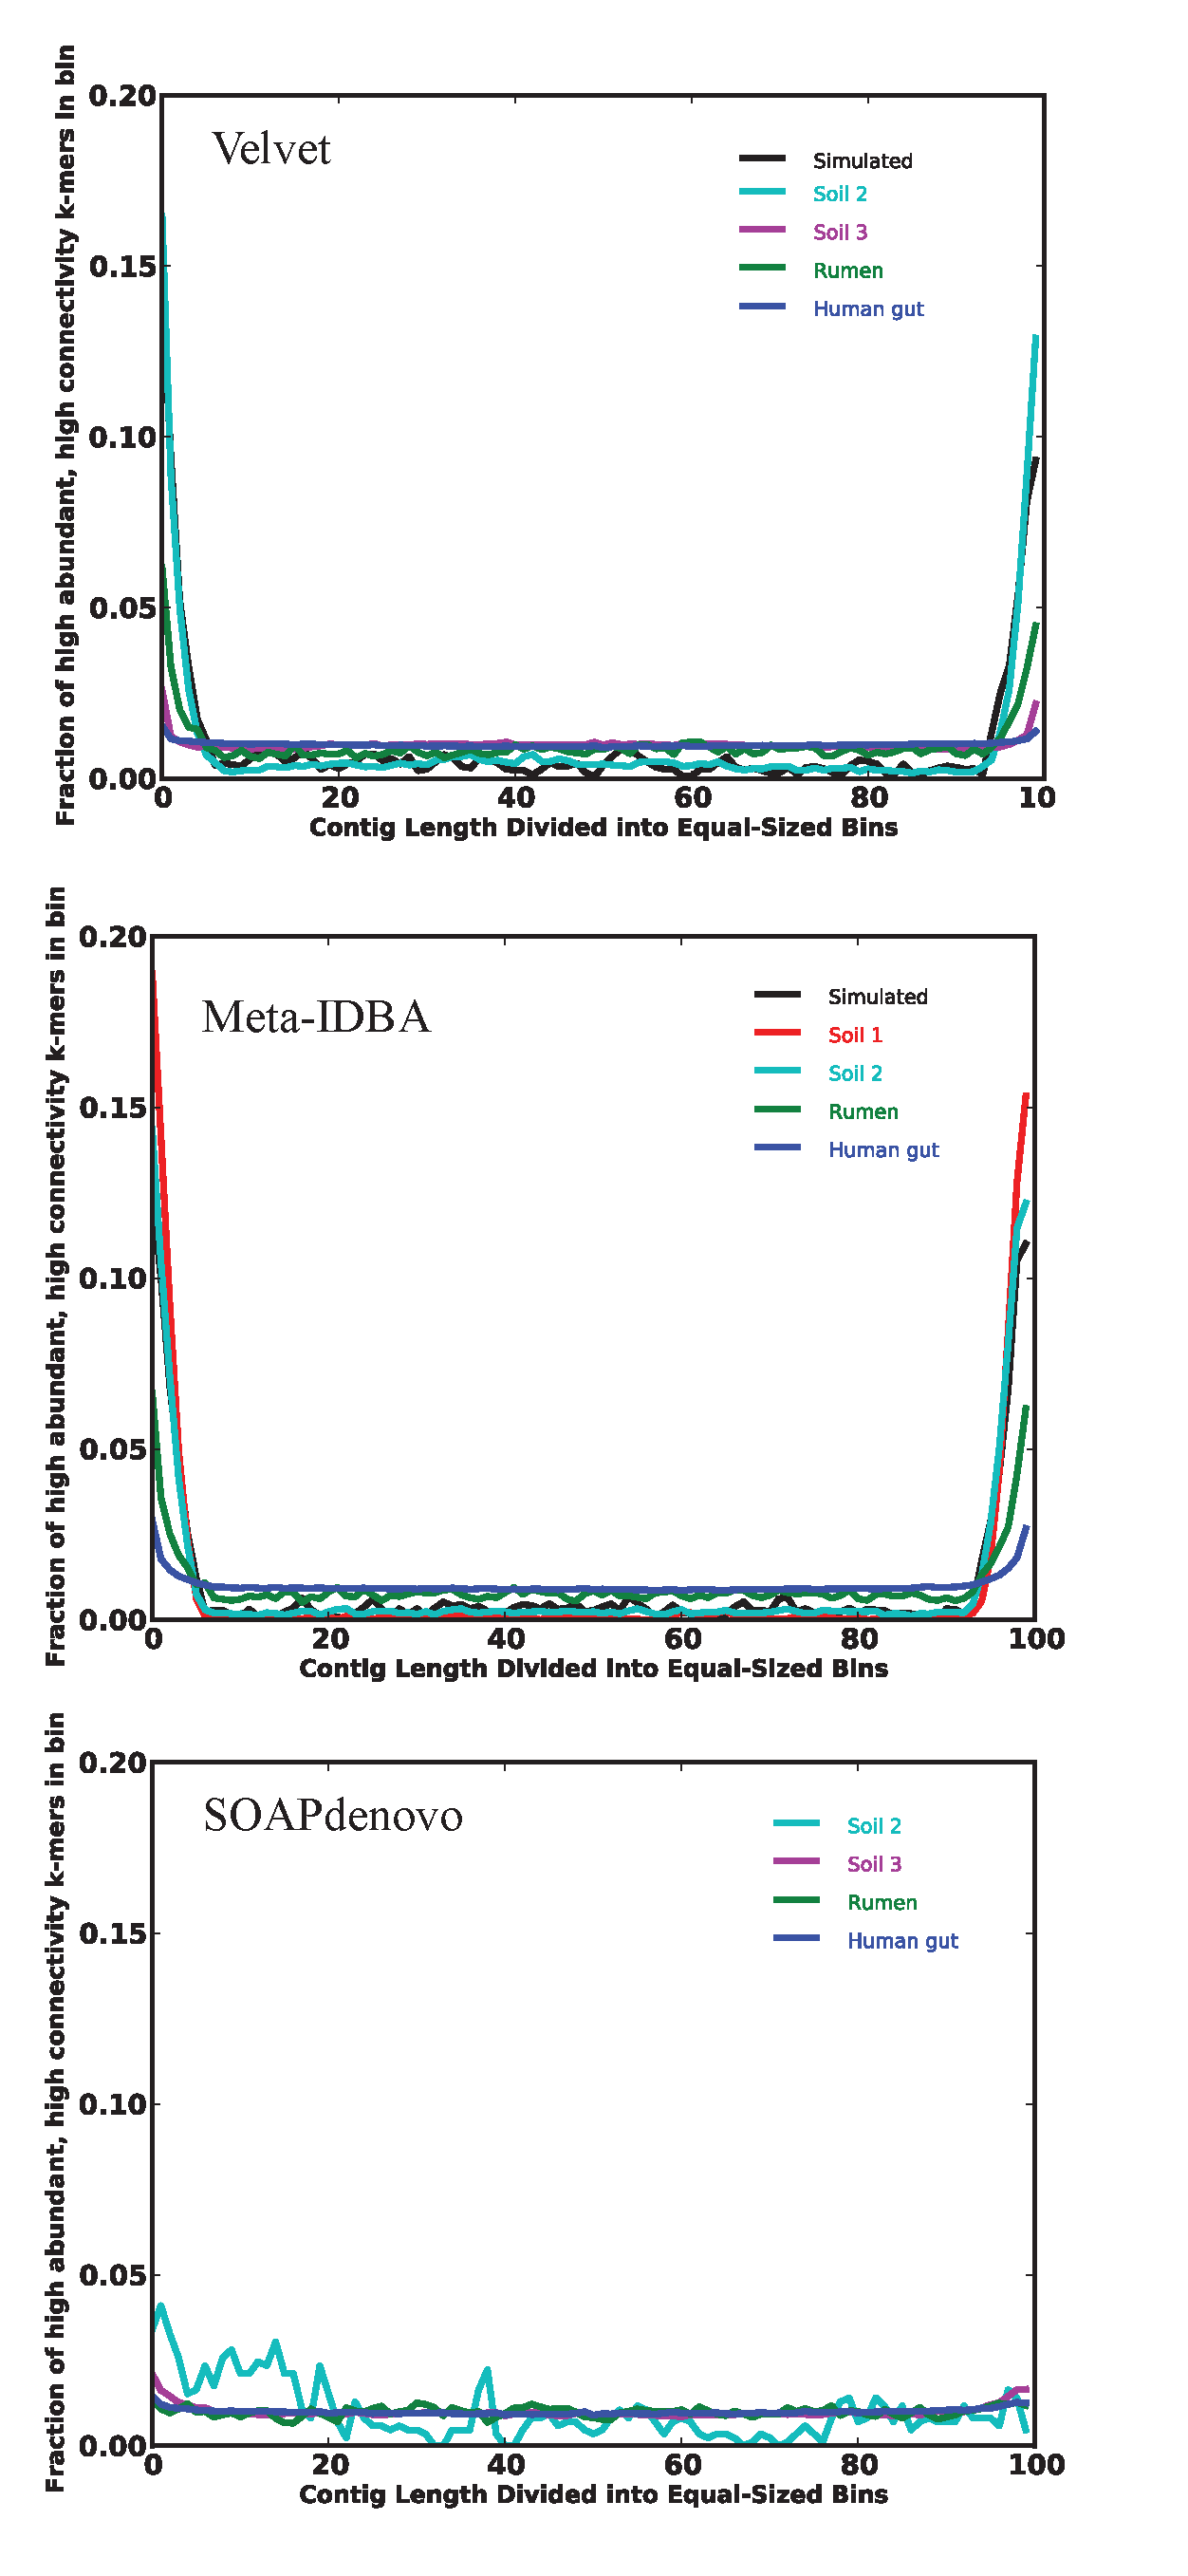
\includegraphics[width=\textwidth,height=\textheight,keepaspectratio]{./Figures/figure3-contigs.pdf}}
\caption{When incorporated into an assembly, abundant (greater than 50 times), highly-connecting sequences (k-mers) were disproportionately present at the ends of contigs.  The total fraction of highly-connecting k-mers which are incorporated into each contig binned region.}
\end{figure}

\begin{figure}
\center{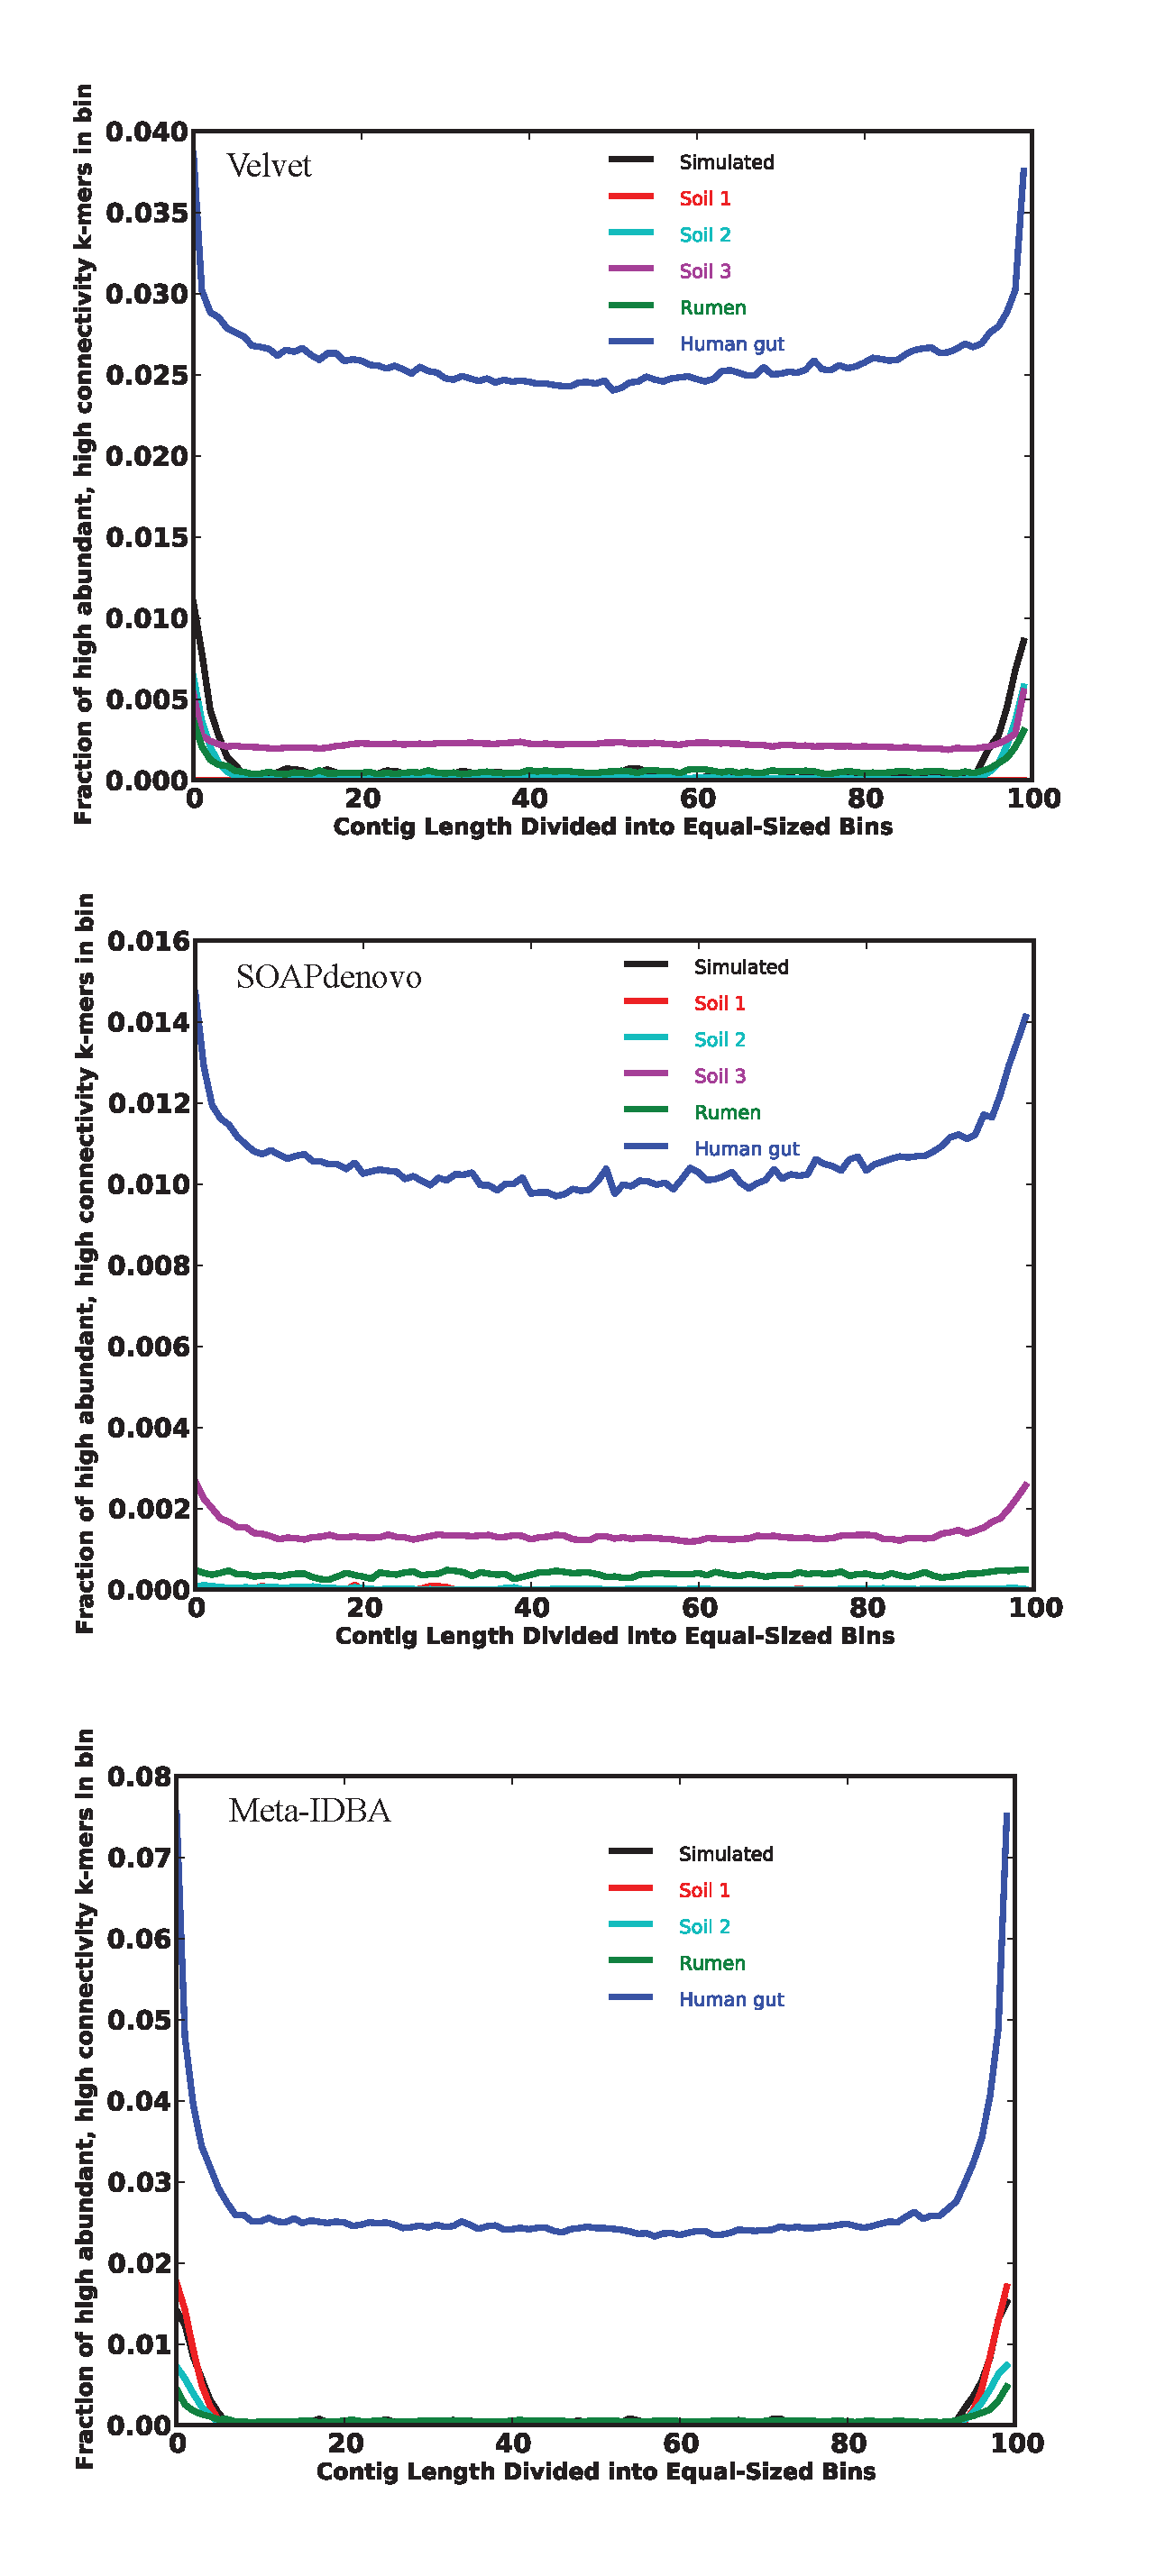
\includegraphics[width=\textwidth,height=\textheight,keepaspectratio]{./Figures/figure4-contigs.pdf}}
\caption{When incorporated into an assembly, abundant (greater than 50 times), highly-connecting sequences (k-mers) were disproportionately present at the ends of contigs.  The total fraction of all k-mers which are identified as high abundant, high connective sequences and incorporated into each contig binned region is shown.}
\end{figure}

\begin{figure}
\center{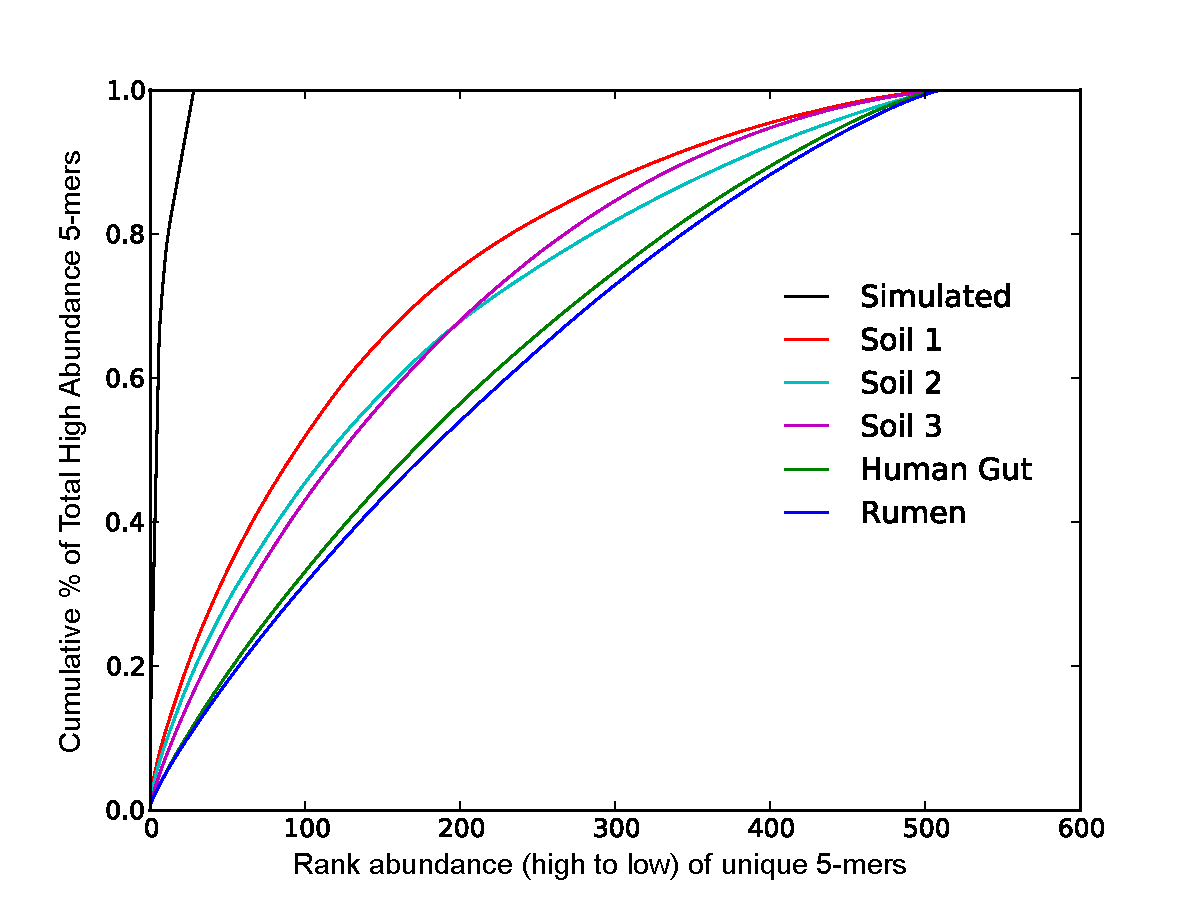
\includegraphics[width=\textwidth,height=\textheight,keepaspectratio]{./Figures/figure5-5mers.pdf}}
\caption{Rank abundance plot of 5-mers present in abundant, highly connective sequences in various datasets.}
\end{figure}
\end{document}









